\documentclass[11pt,a4paper]{article}

\usepackage{../../templates/style}

\begin{document}

\begin{problem}{Dice}{standard input}{standard output}{1 second}{64 megabytes}

กำหนดให้ด้านทั้งหกของลูกเต๋ามีชื่อเรียกดังนี้คือ \textit{บน (Top), หน้า (Front), ซ้าย (Left), หลัง (Back), ขวา (Right) }และ \textit{ล่าง (Bottom)} และกำหนดให้ตำแหน่งเริ่มต้นของลูกเต๋ามีแต้มแต่ละด้านเป็นดังนี้

\begin{figure}[h]
\centering
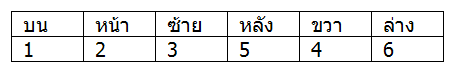
\includegraphics[width=0.7\textwidth]{../latex/img/1006/1006-1.png}
\end{figure}

จากตำแหน่งนี้ลูกเต๋าสามารถหมุนได้หกทิศทาง คือ\textit{หมุนมาทางด้านหน้า (Forward), หมุนไปทางด้านหลัง (Backward), หมุนไปทางซ้าย (Left), หมุนไปทางขวา (Right), หมุนตามเข็มนาฬิกา, (Clockwise) และหมุนทวนเข็มนาฬิกา (Counter clockwise)} ซึ่งการหมุนเหล่านี้มีผลให้แต้มของลูกเต๋าแต่ละด้านเปลี่ยนไป ดังตารางต่อไปนี้

\begin{figure}[h]
\centering
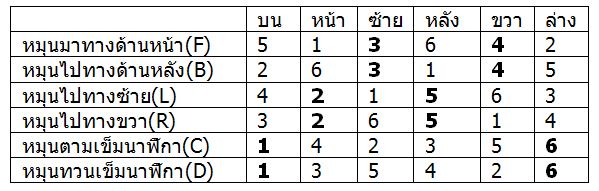
\includegraphics[width=0.7\textwidth]{../latex/img/1006/1006-2.png}
\end{figure}


\underline{\textbf{โจทย์}} จงเขียนโปรแกรมเพื่อรับจำนวนลูกเต๋าและสายอักขระแสดงทิศทางการหมุนของลูกเต๋า แล้วคำนวนหาตำแหน่งสุดท้ายของลูกเต๋าและแสดงแต้มด้านหน้าของลูกเต๋าแต่ละลูก

\InputFile

\textbf{บรรทัดแรก} รับค่า $N$ เป็นจำนวนลูกเต๋า โดยที่ $1 \leq N \leq 6$

\textbf{บรรทัดที่ $2$ ถึง $N+1$} แต่ละบรรทัดรับค่าเป็นสายอักขระแสดงทิศทางการหมุนของลูกเต๋าแต่ละลูก สายอักขระนี้มีความยาวตั้งแต่ $1$ ถึง $1\,000$ ตัวอักษร อักขระแต่ละตัวเป็นอักษรภาษาอังกฤษตัวพิมพ์ใหญ่ตัวใดตัวหนึ่งในหกตัวคือ "B","C","D","F","L","R" (ไม่มีตัวอักษรอื่นนอกจากนี้เลย) ซึ่งใช้แสดงทิศทางการหมุนของลูกเต๋าดังนี้
\begin{itemize}

\item \textbf{F }- หมุนมาทางด้านหน้า (Forward)
\item \textbf{B} - หมุนไปทางด้านหลัง (Backward)
\item \textbf{L} - หมุนไปทางซ้าย (Left)
\item \textbf{R} - หมุนไปทางขวา (Right)
\item \textbf{C} - หมุนตามเข็มนาฬิกา (Clockwise)
\item \textbf{D} - หมุนทวนเข็มนาฬิกา (Counter clockwise)

\end{itemize}

กำหนดให้อักษรตัวแรกในสายอักขระเป็นการหมุนจาก “ตำแหน่งเริ่มต้น”, อักษรตัวที่สองเป็นการหมุนต่อจากที่กำหนดไว้ในอักษรตัวแรก ตัวอย่างเช่นสายอักขระ “CFRL” แทนการหมุนของลูกเต๋าโดยเริ่มจาก “ตำแหน่งเริ่มต้น” ลูกเต๋ามีการหมุนตามเข็มนาฬิกา จากนั้นจึงหมุนมาด้านหน้า แล้วหมุนไปทางขวา จากนั้นจึงหมุนมาทางซ้าย

\OutputFile

\textbf{มีบรรทัดเดียว} ให้แสดงแต้มด้านหน้าของลูกเต๋า ในกรณีที่มีลูกเต๋ามากกว่า $1$ ลูก ให้คั่นค่าแต่ละค่าด้วยเว้นวรรค $1$ วรรค


\Examples

\begin{example}
\exmp{3
D
FFBB
BBFFR}{3 2 2}%
\end{example}

\Source

การแข่งขันคอมพิวเตอร์โอลิมปิก สอวน. ครั้งที่ 2 มหาวิทยาลัยบูรพา

\end{problem}

\end{document}